\newpage

\section{Annexes}

\begin{lstlisting}[language=bash, caption=Récupération du code source du noyau Linux patché]
  git clone git@github.com:intel/uintr-linux-kernel.git
\end{lstlisting}

\begin{lstlisting}[language=bash, caption=Configurer et compiler le noyau]
  # Configurer le noyau sur la machine cible
  cp -v /boot/config-$(uname -r) .config
  make menuconfig

  # Désactiver les clef de signature
  scripts/config --disable SYSTEM_TRUSTED_KEYS
  scripts/config --disable SYSTEM_REVOCATION_KEYS

  # Compiler
  make -j 16
\end{lstlisting}

\begin{lstlisting}[language=bash, caption=Installer le noyau]
  sudo make modules_install
  sudo make install
\end{lstlisting}

\begin{lstlisting}[language=bash, caption=Utiliser le noyau installé]
  # À faire la premier fois
  sudo grub2-mkconfig -o /boot/grub2/grub.cfg

  sudo grubby --set-default /boot/vmlinuz-6.0.0+
\end{lstlisting}

\begin{lstlisting}[language=bash, caption=Lancer les tests \uintr{} du noyau (le noyau doit être installé)]
  make -C tools/testing/selftests TARGETS=uintr run_tests
\end{lstlisting}

\begin{lstlisting}[language=bash, caption=Supprimer le noyau installé]
  sudo grubby --remove-kernel /boot/vmlinuz-6.0.0+
\end{lstlisting}

\begin{figure}[H]
  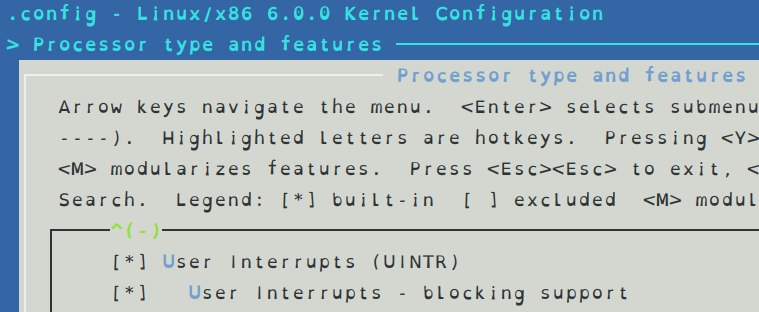
\includegraphics[width=\textwidth]{enableFeaturesInConfigMenu}
  \caption{Activer le support des \uintr{} à la compilation du noyau}
  \label{fig:enableFeaturesInConfigMenu}
\end{figure}

\begin{lstlisting}[language=c, caption=Code récepteur, label={lst:receiverCode}]
  #include <x86gprintrin.h>

  #define VECTOR 6
  bool isOver = 0;

  __attribute__((target("general-regs-only")))
  __attribute__((interrupt))
  void ui_handler(struct __uintr_frame* ui_frame, unsigned long vector) {
    /* Second clock_gettime() here */
    printf("handler invoked (vector: %lld)\n", vector);

    isOver = 1;
  }

  void receiver() {
    if (uintr_register_handler(ui_handler, 0)) {
      perror("interrupt handler register error");
      exit(1);
    }

    _stui();

    int uvec_fd = uintr_vector_fd(VECTOR, 0);
    if (uvec_fd < 0) {
      perror("vector fd error");
      exit(1);
    }

    send_FD_to_sender(uvec_fd);

    while (!isOver) continue;

    if (uintr_unregister_handler(0))
      perror("interrupt handler unregister error");
    close(uvec_fd);
  }
\end{lstlisting}

\begin{lstlisting}[language=c, caption=Code émetteur, label={lst:senderCode}]
  #include <x86gprintrin.h>

  void sender(pid_t targetPid) {
    int uvec_fd = wait_to_receive_FD_from_receiver(targetPid);

    long uipi_index = uintr_register_sender(uvec_fd, 0);
    if (uipi_index < 0) {
      perror("sender register error");
      exit(1);
    }

    /* First clock_gettime() here */
    _senduipi(uipi_index);

    if (uintr_unregister_sender(uipi_index, 0))
      perror("sender unregister error");
    close(uvec_fd);
  }
\end{lstlisting}

\begin{figure}[H]
  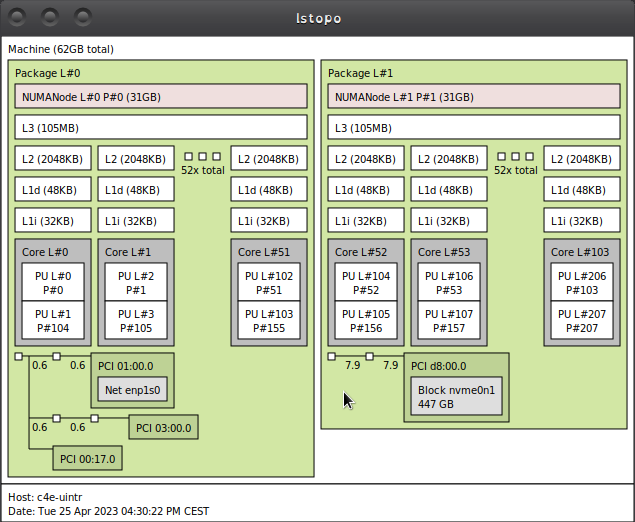
\includegraphics[width=\textwidth]{lstopoC4eUintr}
  \caption{Topologie de la machine fournie par \atos{} obtenue grâce à la commande \emph{lstopo}}
  \label{fig:lstopo}
\end{figure}

\begin{figure}[H]
  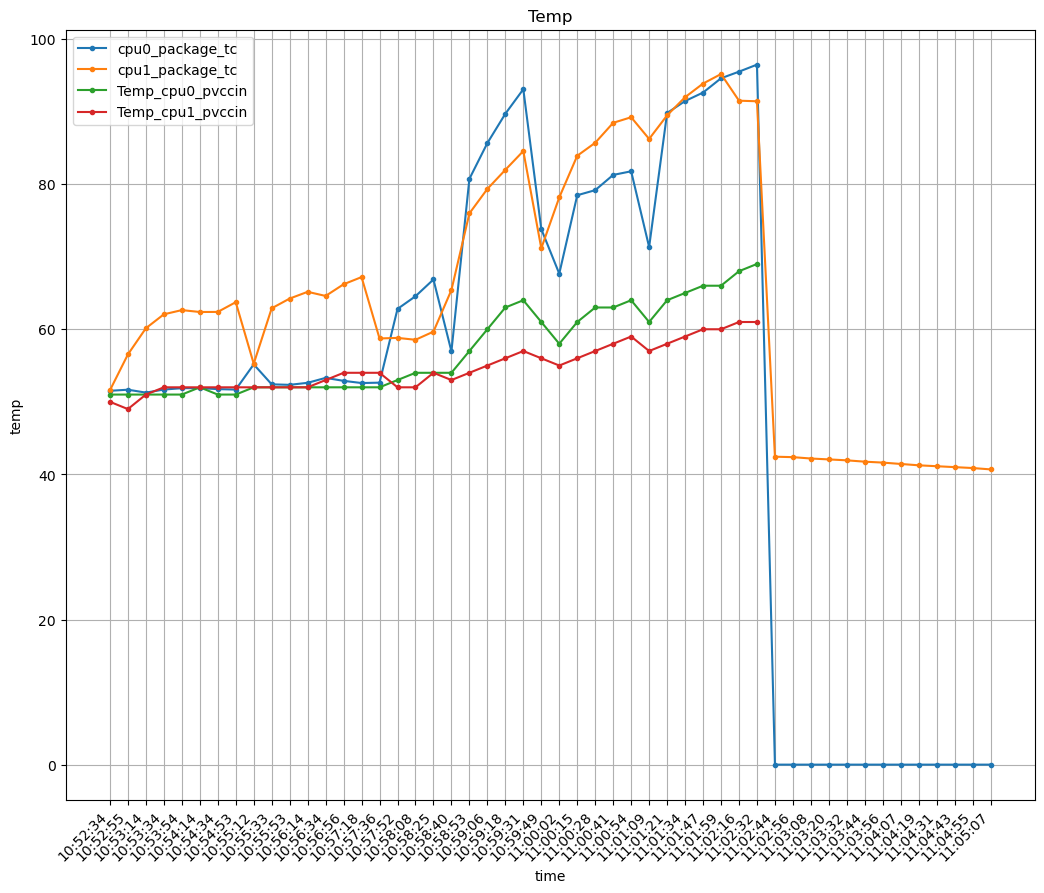
\includegraphics[width=\textwidth]{crashTemp}
  \caption{Courbes de température pour la machine fourni par \atos{}}
  \label{fig:crashTemp}
\end{figure}

\begin{figure}[H]
  \begin{subfigure}{\textwidth}
    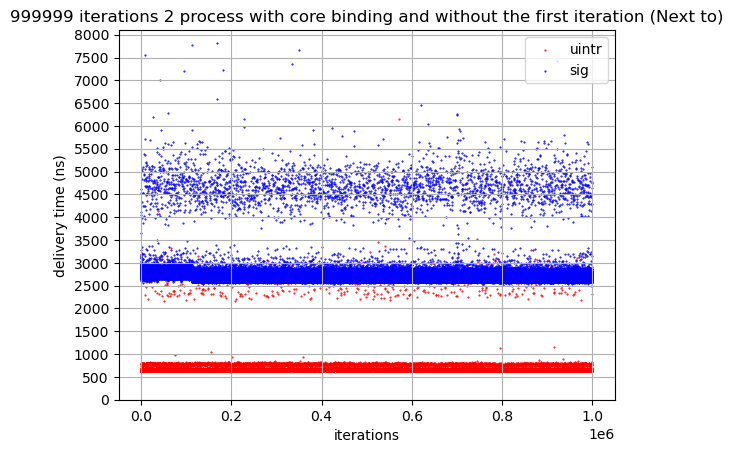
\includegraphics[width=\textwidth]{latency/1e6ProcessNT}
    \caption{}
    \label{subfig:latency1e6ProcessNT}
  \end{subfigure}
  \begin{subtable}{\textwidth}
    \centering
    \begin{tabular}{| l | l | l | l | l | l | l | l |}
      \hline
      &\bf mean &\bf std &\bf min  &\bf 10\% &\bf 50\% &\bf 95\% &\bf max\\
      \hline
      \bf sig   & 2675 & 147 & 2520 & 2620 & 2658 & 2781 & 44311\\
      \hline
      \bf uintr & 651  & 72  & 631  & 642  & 649  & 659  & 46053\\
      \hline
    \end{tabular}
    \caption{}
    \label{tab:latency1e6ProcessNT}
  \end{subtable}
  \caption{Mesures de latence entre deux processus avec un placement proche}
  \label{fig:latency1e6ProcessNT}
\end{figure}

\begin{figure}[H]
  \begin{subfigure}{\textwidth}
    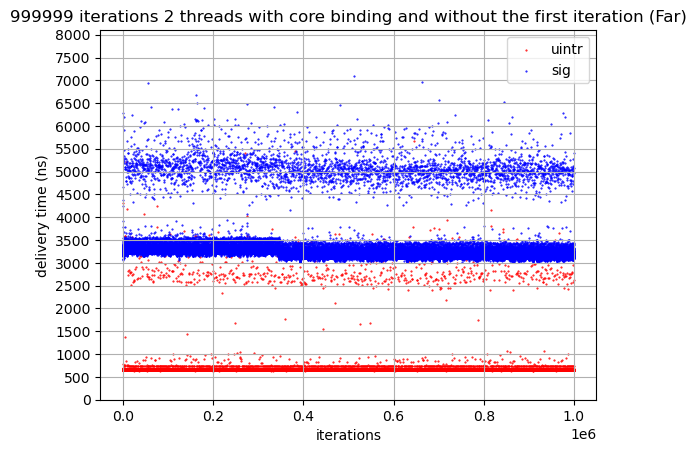
\includegraphics[width=\textwidth]{latency/1e6ThreadsF}
    \caption{}
    \label{subfig:latency1e6ThreadsF}
  \end{subfigure}
  \begin{subtable}{\textwidth}
    \centering
    \begin{tabular}{| l | l | l | l | l | l | l | l |}
      \hline
      &\bf mean &\bf std &\bf min  &\bf 10\% &\bf 50\% &\bf 95\% &\bf max\\
      \hline
      \bf sig   & 3210 & 156 & 3014 & 3141 & 3177 & 3302 & 63690\\
      \hline
      \bf uintr & 654  & 329 & 638  & 648  & 653  & 659  & 325408\\
      \hline
    \end{tabular}
    \caption{}
    \label{tab:latency1e6ThreadsF}
  \end{subtable}
  \caption{Mesures de latence entre deux threads avec un placement éloigné}
  \label{fig:latency1e6ThreadsF}
\end{figure}

\begin{figure}[H]
  \begin{subfigure}{\textwidth}
    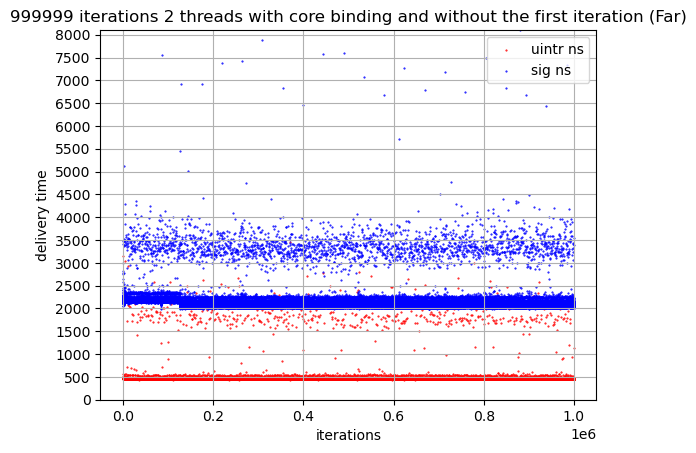
\includegraphics[width=\textwidth]{latency/1e6ThreadsF+TB}
    \caption{}
    \label{subfig:latency1e6ThreadsF-TB}
  \end{subfigure}
  \begin{subtable}{\textwidth}
    \centering
    \begin{tabular}{| l | l | l | l | l | l | l | l |}
      \hline
      &\bf mean &\bf std &\bf min  &\bf 10\% &\bf 50\% &\bf 95\% &\bf max\\
      \hline
      \bf sig   & 2097 & 282 & 1981 & 2064 & 2082 & 2178 & 270625\\
      \hline
      \bf uintr & 455  & 389 & 440  & 450 & 454 & 460 & 388815\\
      \hline
    \end{tabular}
    \caption{}
    \label{tab:latency1e6ThreadsF-TB}
  \end{subtable}
  \caption{Mesures de latence entre deux threads avec un placement éloigné et le turbo boost activé}
  \label{fig:latency1e6ThreadsF-TB}
\end{figure}

\begin{figure}[H]
  \begin{subfigure}{\textwidth}
    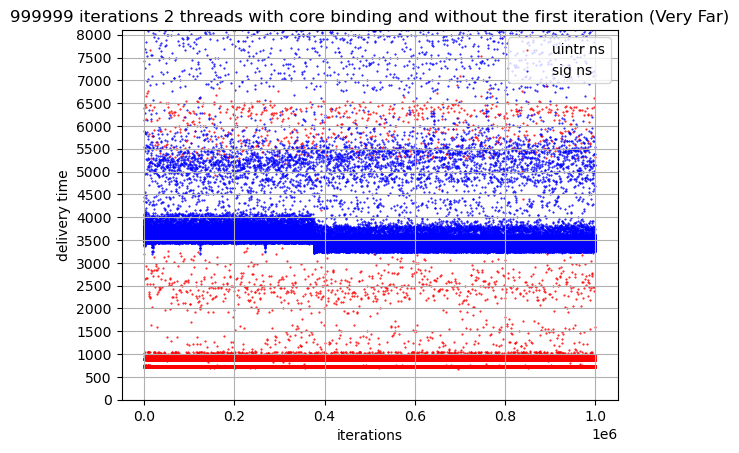
\includegraphics[width=\textwidth]{latency/1e6ThreadsVF+TB}
    \caption{}
    \label{subfig:latency1e6ThreadsVF-TB}
  \end{subfigure}
  \begin{subtable}{\textwidth}
    \centering
    \begin{tabular}{| l | l | l | l | l | l | l | l |}
      \hline
      &\bf mean &\bf std &\bf min  &\bf 10\% &\bf 50\% &\bf 95\% &\bf max\\
      \hline
      \bf sig   & 3520 & 327 & 3189 & 3383 & 3481 & 3678 & 51798\\
      \hline
      \bf uintr & 736  & 159 & 683 & 721 & 725 & 735 & 46787\\
      \hline
    \end{tabular}
    \caption{}
    \label{tab:latency1e6ThreadsVF-TB}
  \end{subtable}
  \caption{Mesures de latence entre deux threads avec un placement très éloigné et le turbo boost activé}
  \label{fig:latency1e6ThreadsVF-TB}
\end{figure}

\begin{figure}[H]
  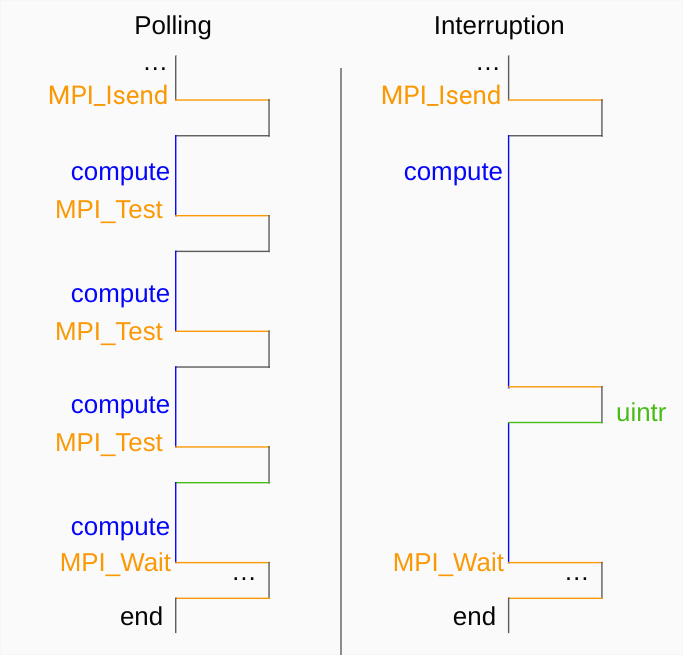
\includegraphics[width=\textwidth]{appPollingVsUintr}
  \caption{Application MPI qui utilise du polling contre une qui utilise des \uintr{}}
  \label{fig:appPollingVsUintr}
\end{figure}
